\documentclass[12pt,aspectratio=169]{beamer}
% Set theme
\usetheme{metropolis}
% Place package includes Here
\usepackage{graphicx}
\usepackage{appendixnumberbeamer}
\usepackage{booktabs}
\usepackage{fontspec}
\defaultfontfeatures{Path=/Library/TeX/Root/texmf-dist/fonts/opentype/public/fontawesome/}
\usepackage{fontawesome}
\usepackage{hyperref}
\usepackage{pythontex}
% % % % % % % % % % % % % % % % % % % % % % % % % % % % % % % % % %
% PythonTeX Bug Fix % % % % % % % % % % % % % % % % % % % % % % % %
% % % % % % % % % % % % % % % % % % % % % % % % % % % % % % % % % % 
% pytexbug fix for context in customcode.
\makeatletter
\renewenvironment{pythontexcustomcode}[2][begin]{%
	\VerbatimEnvironment
	\Depythontex{env:pythontexcustomcode:om:n}%
	\ifstrequal{#1}{begin}{}{%
		\ifstrequal{#1}{end}{}{\PackageError{\pytx@packagename}%
			{Invalid optional argument for pythontexcustomcode}{}
		}%
	}%
	\xdef\pytx@type{CC:#2:#1}%
	\edef\pytx@cmd{code}%
	% PATCH \def\pytx@context{}%
	\pytx@SetContext
	% END PATCH
	\def\pytx@group{none}%
	\pytx@BeginCodeEnv[none]}%
{\end{VerbatimOut}%
\setcounter{FancyVerbLine}{\value{pytx@FancyVerbLineTemp}}%
\stepcounter{\pytx@counter}%
}%
\makeatother
% % % % % % % % % % % % % % % % % % % % % % % % % % % % % % % % % %
\setpythontexcontext{figurewidth=\the\textwidth}
% Other stuff
\setbeamertemplate{caption}{\raggedright\insertcaption\par}
% Title and author
\title{fiasco: a Python interface to the\\CHIANTI atomic database}
\subtitle{Heliophysics Community Python Working Group Meeting\\LASP---Boulder, CO USA}
\date{13 November 2018}
\author{Will Barnes}
\institute{Department of Physics and Astronomy, Rice University\\Houston, TX USA}
\titlegraphic{\hfill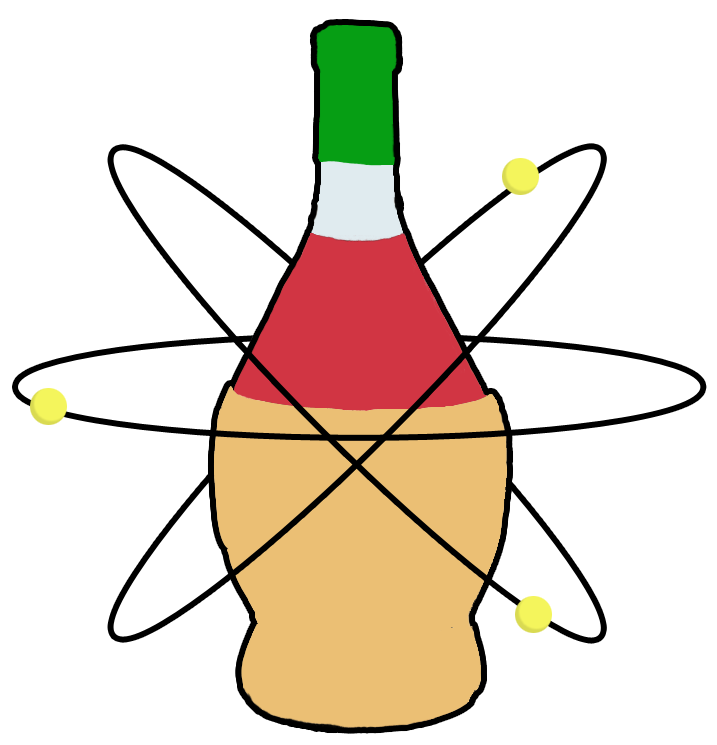
\includegraphics[height=1.6cm]{../figures/fiasco-logo.png}}

% Start Document
\begin{document}

% TeXFigure Manager
\begin{pythontexcustomcode}{py}
import texfigure
texfigure.configure_latex_plots(pytex)
pytex.formatter = texfigure.repr_latex_formatter
import matplotlib.pyplot as plt
\end{pythontexcustomcode}
\begin{pycode}[manager]
manager = texfigure.Manager(pytex, '../figures')
\end{pycode}

% Title
\maketitle

% Contact
{%
\setbeamertemplate{frame footer}{\href{https://wtbarnes.github.io/heliopython-2018-talk}{wtbarnes.github.io/heliopython-2018-talk}}
\begin{frame}{Contact Info}
    \begin{itemize}
        \LARGE
        \item[]\faicon{github} \texttt{wtbarnes}
        \item[]\faicon{twitter} \texttt{wtbarnes\_}
        \item[]\faicon{envelope} \texttt{wtb2@rice.edu} 
        \item[]\faicon{globe} \texttt{wtbarnes.github.io}  
    \end{itemize}
\end{frame}
}

% Content
\begin{frame}
    \begin{figure}
        \centering
        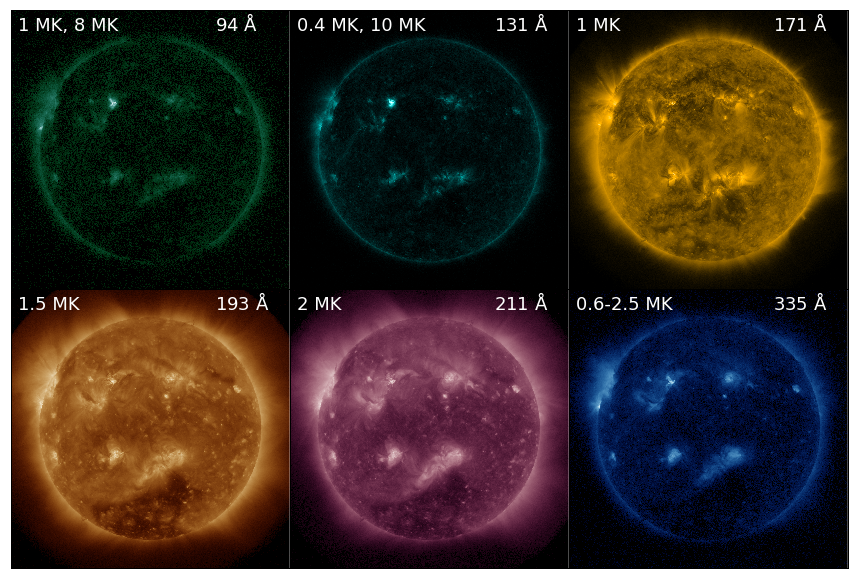
\includegraphics[width=0.9\textwidth]{../figures/aia_all_channels.png}
    \end{figure}
\end{frame}
%%
\section{The CHIANTI Atomic Database}
\begin{frame}[fragile]
    \begin{pycode}[manager]
import fiasco
import astropy.units as u
import roman
import pandas as pd
import plasmapy.atomic
import matplotlib.colors
import seaborn
# Get all ions
ion_list = []
for el_name in fiasco.list_elements():
    el = fiasco.Element(el_name,[1e6]*u.K)
    for ion in el:
        if ion._elvlc is None:
            continue
        ion_list.append({'Element': el.atomic_symbol,
                         'Stage': roman.toRoman(ion.ionization_stage),
                         'Levels': ion[-1].level,})
# Create Table
ion_table = pd.DataFrame(ion_list)
ion_table_pivot = ion_table.pivot('Element','Stage','Levels')
new_indices = sorted(ion_table_pivot.index, key=lambda x:plasmapy.atomic.atomic_number(x))
ion_table_pivot = ion_table_pivot.reindex(new_indices)
ion_table_pivot = ion_table_pivot.reindex_axis(sorted(ion_table_pivot.columns.tolist(),
                                                      key=lambda x:roman.fromRoman(x)),axis=1)
# Create heatmap
fig = plt.figure(figsize=(15,8))
ax=fig.gca()
seaborn.heatmap(ion_table_pivot,
                ax=ax,
                square=False,
                cmap='Blues',
                annot=True,
                fmt='.0f',
                norm=matplotlib.colors.LogNorm(vmin=1,vmax=1e3),
                cbar_kws={'ticks':[1,10,100,1000]},
                mask=ion_table_pivot.isnull(),
                cbar=False)
ax.tick_params(axis='both',which='both',bottom='off',left='off')
fig_chianti_ptable = manager.save_figure('fig_chianti_ptable', fext='.pdf', transparent=True)
fig_chianti_ptable.caption = ''
fig_chianti_ptable.figure_width = r'1.15\textwidth'
fig_chianti_ptable.placement = 't'
    \end{pycode}
    \vspace{-5ex}
    \py[manager]|fig_chianti_ptable|
\end{frame}
%%
\begin{frame}{The CHIANTI Database}
    \begin{itemize}
        \item Began around 1994, collaboration between multiple institutions (U. Cambridge, GMU, NRL, U. Michigan,...)
        \item Data and code distributed freely as tarball or via SSW
        \item Database: ~1.7 GB of plaintext (many thousands of files)
        \item Software
        \begin{itemize}
            \item Parses data; computes rates, population fractions, spectra, etc.
            \item Collection of useful IDL scripts
            \item Lacking: automated tests, documentation, version control, backwards compatibility
            \item \alert{No clear way to contribute code or report bugs!}
        \end{itemize}
        \item \textbf{ChiantiPy} first released in 2006 by K. Dere to provide Python interface to CHIANTI
    \end{itemize}
\end{frame}
%%
\begin{frame}[fragile]{The \emph{fiasco} Package}
\begin{columns}
    \column{0.7\textwidth}
        \begin{itemize}
            \item Scope largely same as IDL tools, ChiantiPy
            \item \alert{Python 3.6+ only}
            \item Licensed under BSD 3-Clause License
            \item Developed openly on \textbf{GitHub}
            \item Documentation builds on \textbf{Read the Docs}
            \item Automated test suite run on \textbf{Travis CI}
            \item Pre-v0.1--conda and pip packages coming soon(ish)
        \end{itemize}
        {\footnotesize
        \begin{pygments}{bash}
> git clone https://github.com/wtbarnes/fiasco.git
> cd fiasco && python setup.py install 
        \end{pygments}
        }
    \column{0.3\textwidth}
        \begin{figure}
            \centering
            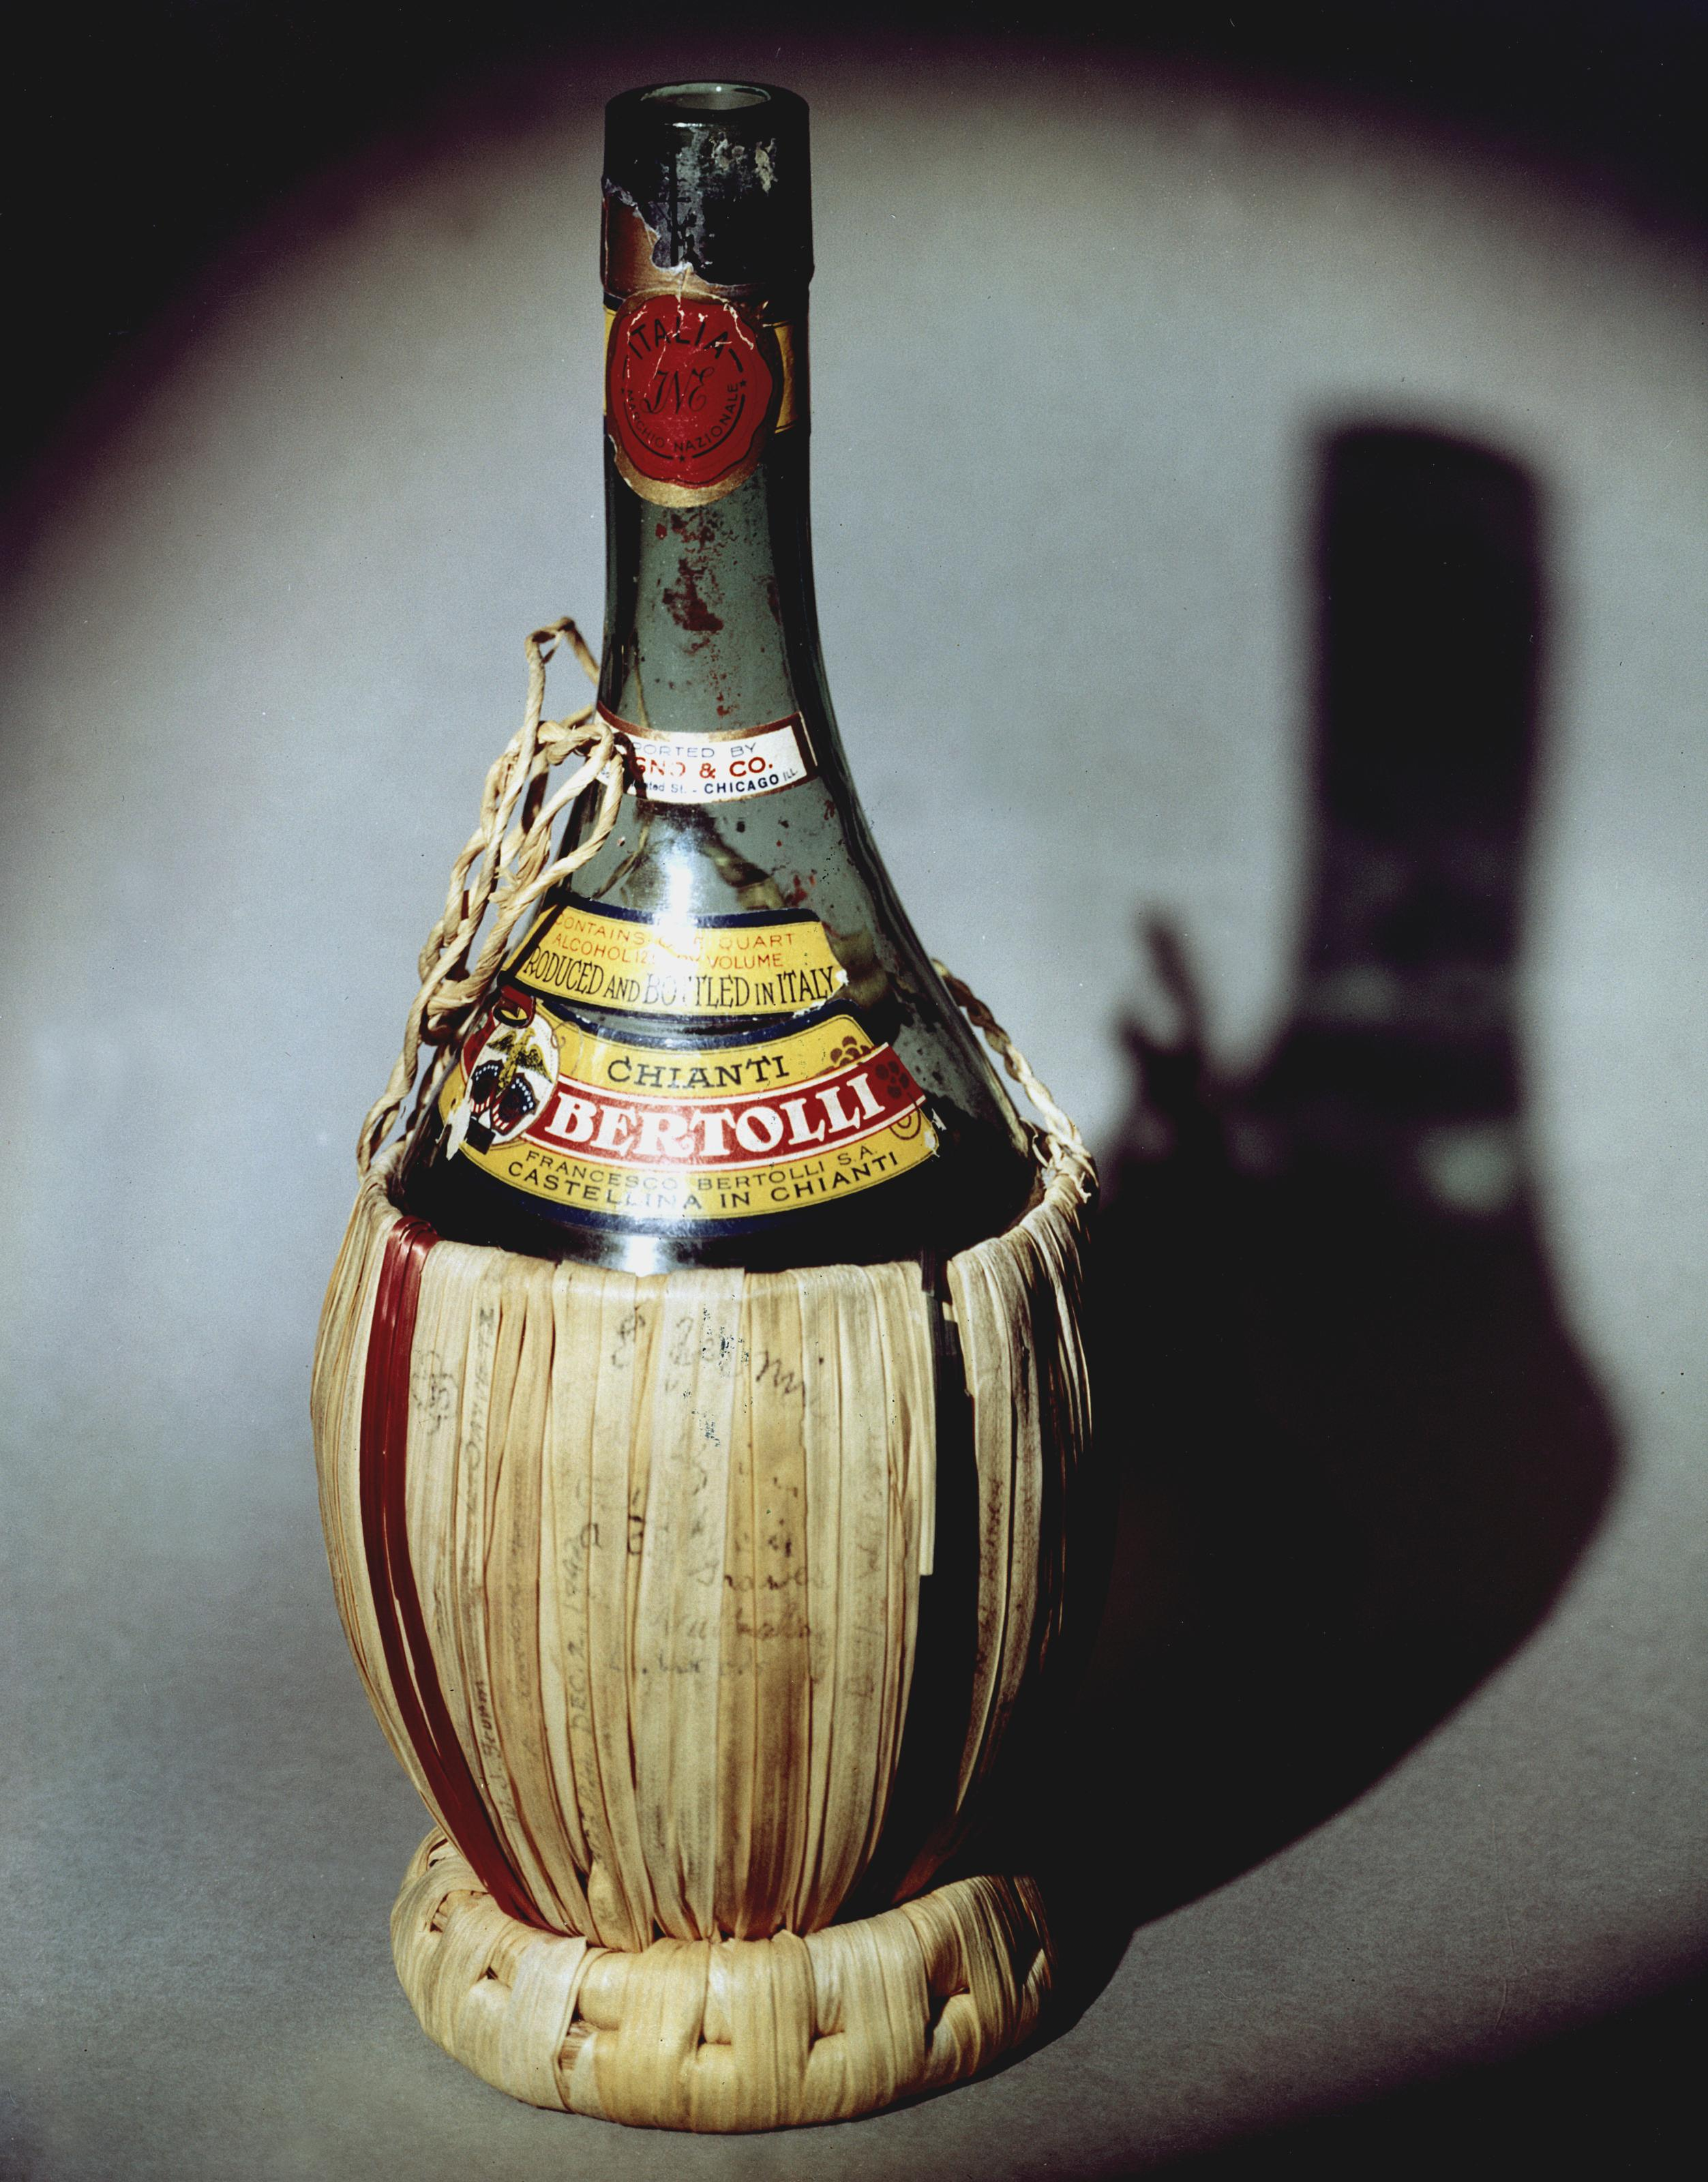
\includegraphics[width=\columnwidth]{../figures/chianti_bottle}
            \caption{}
        \end{figure}
\end{columns}
\end{frame}
%%%
\section{Parsing the Data}
%%
\begin{frame}[fragile]{Many Types of Files...}
    \scriptsize
    \begin{pygments}{bash}
        > tree ~/.fiasco/chianti_dbase/fe
            ├── fe_1
            │   └── fe_1.diparams
            ├── fe_10
            │   ├── fe_10.diparams
            │   ├── fe_10.drparams
            │   ├── fe_10.easplom
            │   ├── fe_10.easplups
            │   ├── fe_10.elvlc
            │   ├── fe_10.fblvl
            │   ├── fe_10.psplups
            │   ├── fe_10.rrparams
            │   ├── fe_10.scups
            │   ├── fe_10.wgfa
            │   └── fe_10_all.scups
            ...
    \end{pygments}    
\end{frame}
%%
\begin{frame}[fragile]{...in Many (Slightly) Different Formats}
    \tiny
    \begin{pygments}{console}
> head -n 5 ~/.fiasco/chianti_dbase/fe/fe_10/fe_10.elvlc
1     3s2 3p5                           2  P    1.5          0.000          0.000
2     3s2 3p5                           2  P    0.5      15683.100      15683.000
3     3s 3p6                            2  S    0.5     289236.000     289236.000
4     3s2 3p4 3d                        4  D    2.5     388713.500     387464.000
5     3s2 3p4 3d                        4  D    3.5     388708.000     387566.000
    \end{pygments}
    \begin{pygments}{console}
> head -n 6 ~/.fiasco/chianti_dbase/fe/fe_10/fe_10.scups
1      2   1.429e-01  -1.000e+00   1.940e-01   12    2   1.798e+01
0.000e+00   4.698e-02   1.097e-01   1.977e-01   3.302e-01   5.520e-01   7.114e-01   8.313e-01   9.249e-01   9.610e-01   9.801e-01   1.000e+00
6.022e+00   5.880e+00   5.690e+00   4.830e+00   3.790e+00   2.400e+00   1.530e+00   9.460e-01   5.190e-01   3.610e-01   2.790e-01   1.940e-01
1      3   2.636e+00   1.371e-01   2.080e-01   12    1   1.246e+00
0.000e+00   1.467e-01   2.949e-01   4.448e-01   5.971e-01   7.541e-01   8.300e-01   8.778e-01   9.149e-01   9.319e-01   9.435e-01   1.000e+00
1.024e+00   1.111e+00   1.198e+00   1.116e+00   9.116e-01   6.303e-01   4.751e-01   3.751e-01   3.030e-01   2.745e-01   2.572e-01   2.080e-01
    \end{pygments}
    \begin{pygments}{console}
> head -n 10 ~/.fiasco/chianti_dbase/fe/fe_10/fe_10.drparams
1
26   10  2.0320e+03  1.0180e+04  4.6380e+04  1.6980e+05  4.4990e+05  7.8800e+05  0.0000e+00  0.0000e+00  0.0000e+00
26   10  5.3350e-04  1.8270e-03  4.8510e-03  2.7100e-02  8.2260e-02  3.1470e-01  0.0000e+00  0.0000e+00  0.0000e+00
-1
file:  fe_10.drparams
parameters for dielectronic recombination rate coefficients
Determined from the coefficients listed at:
http://amdpp.phys.strath.ac.uk/tamoc/DATA/RR/
These calculations have been performed by a collaboration of researchers at:
Auburn University, Rollins College, and the University of Strathclyde.
    \end{pygments}
\end{frame}
%%
\begin{frame}{Parser Factory}
    \begin{columns}
        \column{0.6\textwidth}
            \begin{itemize}
                \item Many filetypes with many "quirks"
                \item \texttt{ParserFactory} metaclass creates parser classes "on the fly"
                \item Filetype determines parser class using a \emph{factory pattern}
                \item In most simple case, parser class just provides
                \begin{itemize}
                    \item[-] headings
                    \item[-] units
                    \item[-] types
                    \item[-] descriptions
                \end{itemize}
            \end{itemize}
        \column{0.4\textwidth}
            \includegraphics[width=0.9\columnwidth]{../figures/parser_inheritance_diagram.pdf}
    \end{columns}
\end{frame}
%%
\begin{frame}[fragile]{Parser Factory}
\footnotesize
\begin{pyconsole}
from fiasco.io import Parser
p = Parser('fe_16.elvlc')
p.parse()[:3]
type(p)
\end{pyconsole}
\end{frame}
\begin{frame}[fragile]{Parser Factory}
\scriptsize
\begin{pyconsole}
from fiasco.io import Parser
p = Parser('al_6.psplups')
p.parse()[:3]
type(p)
print(p.parse().meta['footer'])
\end{pyconsole}
\end{frame}
%%
\begin{frame}{HDF5 as a Database}
    \begin{itemize}
        \item Repeatedly parsing plaintext files is annoying
        \item \textbf{Instead, use HDF5!}
        \begin{itemize}
            \item[-] Hierarchical Data Format
            \item[-] Entire filetree in a single binary blob
            \item[-] Python interface via \texttt{h5py} package 
        \end{itemize}
        \item Easily slice and select parts of data that you need
        \item Easily store \alert{metadata alongside the data}
    \end{itemize}
\end{frame}
\begin{frame}[fragile]{HDF5 as a Database}
    \footnotesize
    \begin{pyconsole}
import h5py; from fiasco.io import Parser
p = Parser('fe_16.elvlc'); table = p.parse()
with h5py.File('chianti.h5', 'w') as hf:
    p.to_hdf5(hf, table)

from fiasco import DataIndexer
d = DataIndexer('chianti.h5', 'fe/fe_16/elvlc')
d.footer
d.version
'E_obs' in d
d['E_obs'][:3]
    \end{pyconsole}
\end{frame}
%%%
\section{The \texttt{Ion} Class}
%%
\begin{frame}[fragile]{The \texttt{Ion} Class}
    \footnotesize
    \begin{pyconsole}[ion_class]
from fiasco import Ion
import numpy as np; import astropy.units as u
t = np.logspace(4, 9, 100)*u.K
ion = Ion('Fe 16', temperature=t)
# Or
ion = Ion('Fe +15', t); ion = Ion('iron 16', t)
ion.element_name,ion.atomic_symbol,ion.atomic_number
ion.ion_name,ion.ionization_stage,ion.charge_state
type(ion._elvlc) # Access raw data
ion._elvlc['E_obs'][:3]
    \end{pyconsole}
\end{frame}
%%
\begin{frame}[fragile]{The \texttt{Ion} Class: Energy Levels and Transitions}
    \small
    \begin{pyconsole}[ion_class]
ion[0]
ion[1].level,ion[1].configuration
[level.energy.to(u.eV) for level in ion]
ion.transitions.wavelength[:3]
ion.transitions.delta_energy[:3].to(u.eV)
    \end{pyconsole}
\end{frame}
%%
\begin{frame}[fragile]{The \texttt{Ion} Class: Derived Quantities}
    \scriptsize
    \begin{pyconsole}[ion_class]
ion.ionization_rate()[:3]
ion.recombination_rate()[:3]
    \end{pyconsole}
    \begin{pycode}[manager]
import fiasco
import numpy as np; import astropy.units as u
t = np.logspace(4, 9, 100)*u.K
ion = fiasco.Ion('Fe 16', temperature=t)
fig = plt.figure(figsize=(12,5))
ax = fig.gca()
# Ionization Rate
ax.plot(t,ion.ionization_rate(),label='Ionization',color='C0',ls='-')
ax.plot(t,ion.direct_ionization_rate(),color='C0',ls='--',label='Direct Ionization')
ax.plot(t,ion.excitation_autoionization_rate(),color='C0',ls=':',label='Excitation Autoionization')
# Recombination rate
ax.plot(t,ion.recombination_rate(),label='Recombination',color='C1',ls='-')
ax.plot(t,ion.radiative_recombination_rate(),color='C1',ls='--',label='Radiative Recombination')
ax.plot(t,ion.dielectronic_recombination_rate(),color='C1',ls=':',label='Dielectronic Recombination')
ax.set_xscale('log')
ax.set_yscale('log')
ax.set_ylim(1e-12,1e-9)
ax.set_xlim(1e4,1e9)
ax.set_xlabel(f'$T$ [{ion.temperature.unit.to_string("latex")}]')
ax.set_ylabel(f'Rate [{ion.ionization_rate().unit.decompose().cgs.to_string("latex")}]')
ax.legend(loc=3)
fig_ion_rates = manager.save_figure('fig_ion_rates', fext='.pdf', transparent=True)
fig_ion_rates.caption = ''
fig_ion_rates.figure_width = r'\textwidth'
fig_ion_rates.placement = 't'
    \end{pycode}
    \vspace{-5ex}
    \py[manager]|fig_ion_rates|
\end{frame}
%%%
\section{Dealing with Multiple Ions}
\begin{frame}[fragile]{The \texttt{Element} Class}
    \begin{pyconsole}[ion_class]
from fiasco import Element
fe = Element('iron', temperature=t)
fe.element_name,fe.atomic_number,fe.atomic_symbol
fe.abundance
type(fe[0])
[ion.ion_name for ion in fe][:5]
    \end{pyconsole}
\end{frame}
%%
\begin{frame}[fragile]{The \texttt{Element} Class}
    \begin{pyconsole}[ion_class]
ioneq = fe.equilibrium_ionization()
    \end{pyconsole}
    \begin{pycode}[manager]
from fiasco import Element
import numpy as np; import astropy.units as u
t = np.logspace(4, 9, 100)*u.K
fe = Element('iron',t)
ioneq = fe.equilibrium_ionization()
fig = plt.figure(figsize=(12,5))
ax = fig.gca()
for ion in fe:
    ax.plot(fe.temperature, ioneq[:,ion.charge_state], color=f'C{ion.charge_state%10}')
ax.set_xscale('log')
ax.set_xlabel(f'$T$ [{fe.temperature.unit.to_string("latex")}]')
ax.set_ylabel(r'Population Fraction')
ax.set_xlim(t[0].value,t[-1].value)
fig_ioneq = manager.save_figure('fig_ioneq', fext='.pdf', transparent=True)
fig_ioneq.caption = ''
fig_ioneq.figure_width = r'1.1\textwidth'
fig_ioneq.placement = 't'
    \end{pycode}
    \vspace{-5ex}
    \py[manager]|fig_ioneq|
\end{frame}
%%c
\begin{frame}[fragile]{Combining Ions}
    \begin{itemize}
        \item General collection of ions
        \item Useful for computing spectra and radiative loss curves
    \end{itemize}
    \begin{pyconsole}[ion_class]
fe_5 = Ion('Fe 5', t)
fe_13 = Ion('Fe 13', t)
fe_18 = Ion('Fe 18', t)
from fiasco import IonCollection
c = IonCollection(fe_5,fe_13,fe_18)
# Or
c = fe_5 + fe_13 + fe_18
# Or
c = Ion('H 1', t) + Element('iron', t)
    \end{pyconsole}
\end{frame}
%%
\begin{frame}[fragile]{Combining Ions}
    \footnotesize
    \begin{pyverbatim}
r = IonCollection(fe_5).radiative_loss([1e9]*u.cm**(-3))
    \end{pyverbatim}
    \begin{pycode}[manager]
from fiasco import Ion, IonCollection
import numpy as np
import astropy.units as u
t = np.logspace(4, 9, 100)*u.K
fe_5 = Ion('Fe 5', t)
r = IonCollection(fe_5).radiative_loss([1e9]*u.cm**(-3))
fig = plt.figure(figsize=(12,5))
ax = fig.gca()
ax.plot(t,r)
ax.set_xscale('log')
ax.set_yscale('log')
ax.set_ylim(1e-30,1e-22)
ax.set_xlabel(f'$T$ [{fe.temperature.unit.to_string("latex")}]')
ax.set_ylabel(f'Radiative Loss [{r.unit.to_string("latex")}]')
fig_radloss = manager.save_figure('fig_radloss', fext='.pdf', transparent=True)
fig_radloss.caption = ''
fig_radloss.figure_width = r'\textwidth'
fig_radloss.placement = 't'
    \end{pycode}
    \vspace{-3ex}
    \py[manager]|fig_radloss|
\end{frame}
%%
\begin{frame}[fragile]{Combining Ions}
    \footnotesize
    \begin{pyverbatim}
r = (fe_5 + fe_13).radiative_loss([1e9]*u.cm**(-3))
    \end{pyverbatim}
    \begin{pycode}[manager]
fe_13 = Ion('Fe 13', t)
r = (fe_5 + fe_13).radiative_loss([1e9]*u.cm**(-3))
fig = plt.figure(figsize=(12,5))
ax = fig.gca()
ax.plot(t,r)
ax.set_xscale('log')
ax.set_yscale('log')
ax.set_ylim(1e-30,1e-22)
ax.set_xlabel(f'$T$ [{fe.temperature.unit.to_string("latex")}]')
ax.set_ylabel(f'Radiative Loss [{r.unit.to_string("latex")}]')
fig_radloss_2 = manager.save_figure('fig_radloss_2', fext='.pdf', transparent=True)
fig_radloss_2.caption = ''
fig_radloss_2.figure_width = r'\textwidth'
fig_radloss_2.placement = 't'
    \end{pycode}
    \vspace{-3ex}
    \py[manager]|fig_radloss_2|
\end{frame}
%%
\begin{frame}[fragile]{Combining Ions}
    \footnotesize
    \begin{pyverbatim}
r = (fe_5 + fe_13 + fe_18).radiative_loss([1e9]*u.cm**(-3))
    \end{pyverbatim}
    \begin{pycode}[manager]
fe_18 = Ion('Fe 18', t)
r = (fe_5 + fe_13 + fe_18).radiative_loss([1e9]*u.cm**(-3))
fig = plt.figure(figsize=(12,5))
ax = fig.gca()
ax.plot(t,r)
ax.set_xscale('log')
ax.set_yscale('log')
ax.set_ylim(1e-30,1e-22)
ax.set_xlabel(f'$T$ [{fe.temperature.unit.to_string("latex")}]')
ax.set_ylabel(f'Radiative Loss [{r.unit.to_string("latex")}]')
fig_radloss_3 = manager.save_figure('fig_radloss_3', fext='.pdf', transparent=True)
fig_radloss_3.caption = ''
fig_radloss_3.figure_width = r'\textwidth'
fig_radloss_3.placement = 't'
    \end{pycode}
    \vspace{-3ex}
    \py[manager]|fig_radloss_3|
\end{frame}
%%%
\section{Looking Forward}
%%
\begin{frame}{Remote Data Access}
    \begin{figure}
        \centering
        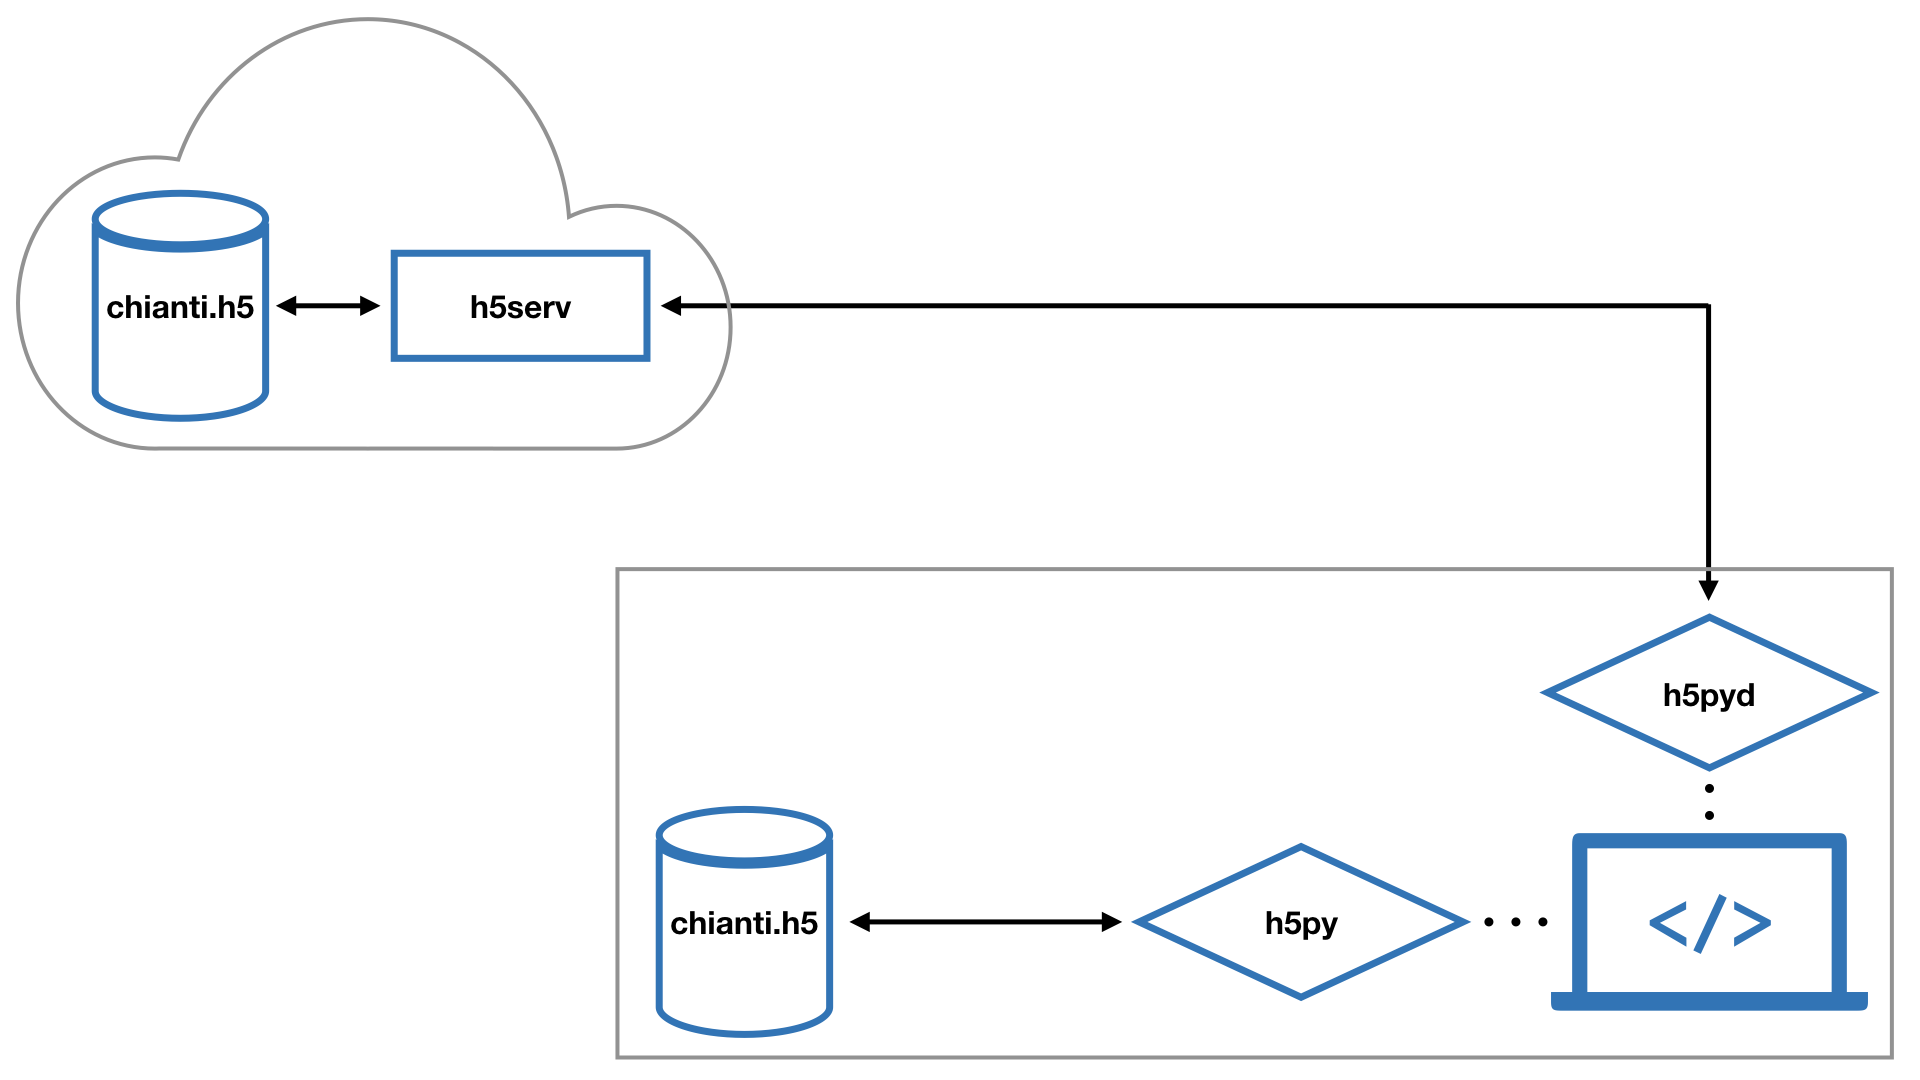
\includegraphics[width=0.95\textwidth]{../figures/cloud_diagram.png}
    \end{figure}
\end{frame}
%%
\begin{frame}[allowframebreaks]{Roadmap}
    \begin{itemize}
        \item Features
        \begin{itemize}
            \item[-] Continuum emission (bremsstrahlung, free-bound)
            \item[-] Parse older versions of the database
            \item[-] Spectra
            \item[-] Radiative losses 
            \item[-] Remote data
        \end{itemize}
        \item Infrastructure
        \begin{itemize}
            \item[-] \textbf{Testing:} Rigourous comparison against CHIANTI IDL
            \item[-] \textbf{Testing:} Improved coverage overall
            \item[-] \textbf{Docs:} More thorough tutorial
        \end{itemize}
        \item Meta
        \begin{itemize}
            \item[-] Bring under project umberella---SunPy? CHIANTI? Heliopython?
            \item[-] Encourage contributions from community 
            \item[-] Integrate with CHIANTI team 
            \item[-] Interoperability between other atomic datasets (e.g. AtomDB, Cloudy) 
        \end{itemize}
    \end{itemize}
\end{frame}
%%%
{%
\setbeamertemplate{frame footer}{\href{https://wtbarnes.github.io/heliopython-2018-talk}{wtbarnes.github.io/heliopython-2018-talk}}
\begin{frame}{Resources}
    \begin{itemize}
        \LARGE
        \item[]\faicon{github} \texttt{wtbarnes/fiasco}
        \item[]\faicon{book} \texttt{fiasco.readthedocs.io}
        \item[]\faicon{globe} \texttt{chiantidatabase.org}   
    \end{itemize}
\end{frame}
}
%%
\begin{frame}{Acknowledgement}
    \begin{itemize}
        \item CHIANTI Team
        \item Ken Dere (ChiantiPy)
        \item SunPy Project (Stuart Mumford, David Pérez-Suárez)
        \item PlasmaPy Project (Nick Murphy, Drew Leonard)
        \item Stephen Bradshaw (Rice)
    \end{itemize}
\end{frame}
\end{document}
